\documentclass{article}
\usepackage[utf8]{inputenc}
\usepackage[english]{babel}

\usepackage{comment}
\usepackage{hyperref}
\usepackage{amsmath}
\usepackage{graphicx}
\usepackage{geometry}
\usepackage[style=alphabetic]{biblatex}
\addbibresource{refs.bib}


%% ponemos el nombre de la carpeta (antes de .bib) donde pegaremos nuestra bibliografäia en formato bibtex. Ver la carpeta al lado derecho que se llama refs.bib 



\title{Ideas de Investigación STEM GNOMON}
\author{INTEGRANTES SEMILLERO}
\date{May 2021}
    

    
\begin{document}



\maketitle

\begin{abstract}
        Este artículo describe las posibles ideas de investigación de interes profesional. Pretendo elegir una de ellas y crear a una pregunta de investigación a partir de un buen estado del arte. 
\end{abstract}

\tableofcontents


\section{Introduction}
\subsection{Ideas de Investigación}

%% Primera tarea, enumerar las ideas y nombrarlas de forma corta.

Las ideas de ivestigación son:
        \begin{enumerate} 
            \item{Aquí titulan la idea 1}
            \item{Aquí titulan la idea 2}
            \item{Aquí titulan la idea 3}
            \item{Aquí titulan la idea 4}
        \end{enumerate}
        
        
\subsubsection{Idea de investigación 1}%% aquí plantearemos mas adelante el problema de la idea de investigación 1; que decidiremos.

\subsubsection{Estado del Arte de la Idea de investigación 1} aquí escribiremos sobre las investigaciones que se han preguntado lo mismo que yo me he preguntado con mi idea de investigación. Hablaremos de forma corta y concisa sobre los métodos usados y sobre los resultados obtenidos, conclusiones y preguntas que quedan abiertas aún en cada artículo revisado. Ademas la citaremos con el comando: \cite{ctan} 
\cite{knuth-acp}
\cite{dirac}

%% las respectivas palabras clave que aparecen dentro de las llaves, luego de del comando cite, deben estar pegadas previamente en el archivo refs.bib. y es la primera palabra que aparece antes de la primera coma; dentro de cada bibliografía en formato plano.

\subsubsection{Metodología idea 1} %%Metodología que voy a usar para responder

\begin{figure}[h]
    \centering
        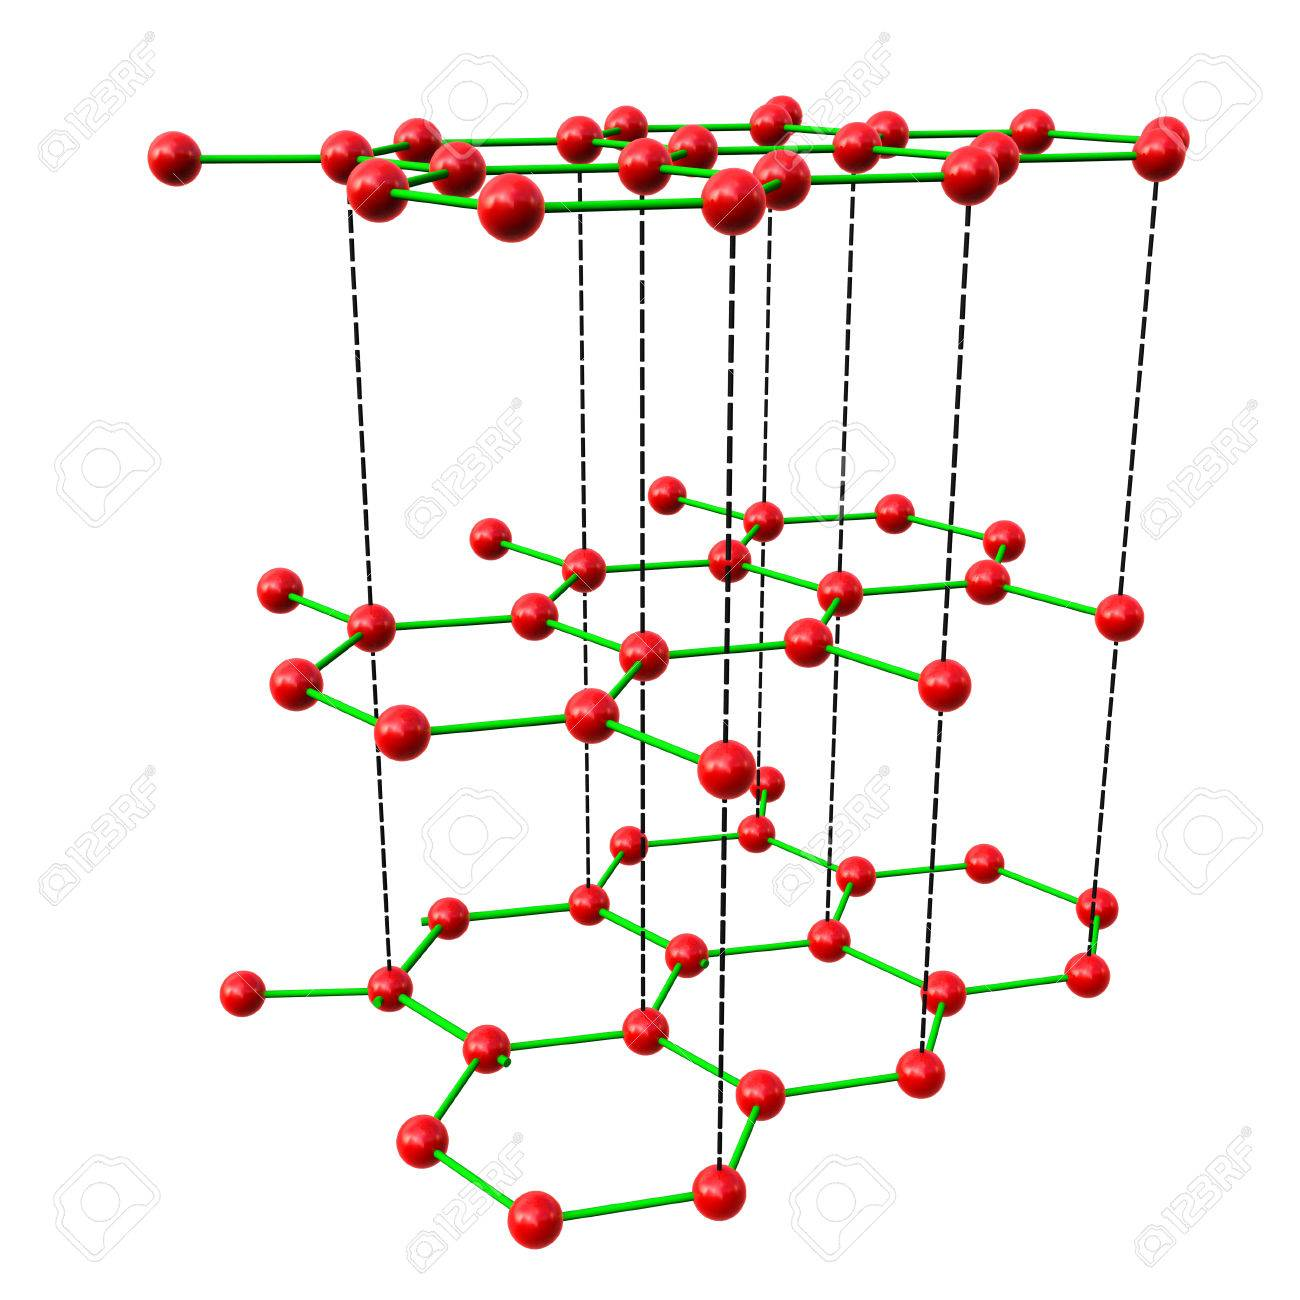
\includegraphics[height=3cm]{images/39620810-la-estructura-de-grafito.jpg}
    \caption{Esté es una imagen que me ayuda a describir mejor la idea de investigación para explicársela a mis colegas investigadores del semillero o de otras universidades del mundo. }
    \label{fig:fg1}
\end{figure}


\section{Materials and methods}
La fibración de Hopf se expresa como sigue:
\vspace{0.2in}

    \begin{equation}
         S^{1}\hookrightarrow S^{3} \xrightarrow{p}S^{2}
         \label{eq1}
    \end{equation}
    
    

\section{Results}

Esta es seccíon x.Esta es seccíon x.Esta es seccíon x.Esta es seccíon x.Esta es seccíon x.Esta es seccíon x.Esta es seccíon x.Esta es seccíon x.Esta es seccíon x.vEsta es seccíon x.Esta es seccíon x.Esta es seccíon x.Esta es seccíon x.Esta es seccíon x.Esta es seccíon x.Esta es seccíon x.Esta es seccíon x.

\section{Discussion}


\section{Conclusions}

\medskip
\printbibliography[title={Bibliography}]

\end{document}
